% Top view of the floor frame for ROME_lab_procedure.tex (Plan 3 Task 5).
% Schematic, not to scale. No measured value is drawn: the origin location (TRACKER Q-D2), the
% tracked region (Part C C9.6) and the start marks (Part C C11) are not measured yet.
% Frame: spec docs/2026-11-18-rome-sim-to-lab-plan.md step 10 (origin = target, x radial,
% y in-track, z up, heading from +x). Heading symbol theta_v from Research/writing_rules/NOTATION.md
% (the task brief wrote psi, which NOTATION.md reserves for the constraint function).
% Drawn x right, y up, so that z up points out of the page (right-handed), CLAUDE.md section 28.
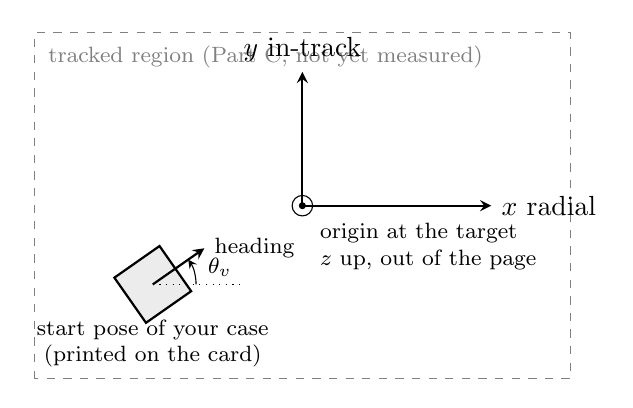
\begin{tikzpicture}[>=stealth]
  % tracked region, not measured
  \draw[dashed, gray] (-3.4,-2.2) rectangle (3.4,2.2);
  \node[gray, anchor=north west, font=\footnotesize] at (-3.35,2.15) {tracked region (Part C, not yet measured)};
  % floor frame
  \draw[->, thick] (0,0) -- (2.4,0) node[right] {$x$ radial};
  \draw[->, thick] (0,0) -- (0,1.7) node[above] {$y$ in-track};
  \draw (0,0) circle (0.13);
  \fill (0,0) circle (0.045);
  \node[anchor=north west, font=\footnotesize, align=left] at (0.1,-0.1) {origin at the target\\$z$ up, out of the page};
  % schematic robot at a start pose
  \begin{scope}[shift={(-1.9,-1.0)}, rotate=35]
    \draw[thick, fill=gray!15] (-0.35,-0.35) rectangle (0.35,0.35);
    \draw[->, thick] (0,0) -- (0.8,0) node[right, font=\footnotesize] {heading};
  \end{scope}
  \draw[dotted] (-1.9,-1.0) -- (-0.8,-1.0);
  \draw[->] (-1.35,-1.0) arc (0:35:0.55);
  \node[font=\footnotesize] at (-1.05,-0.78) {$\theta_v$};
  \node[font=\footnotesize, align=center] at (-1.9,-1.75) {start pose of your case\\(printed on the card)};
\end{tikzpicture}
